% \documentclass{report}
% 
% \usepackage{fancyhdr}
\usepackage{fourier-orns}
\usepackage{hyperref}%% To refrence links / jumps
\usepackage{chngcntr} %% For some extra counters numberings
\usepackage[a4paper, right = 0.5in, left = 0.5in,top = 1in , bottom = 1in]{geometry}
\usepackage{etoolbox} %% Provides like a language for advanced customization
\usepackage{datetime} %% For dates of course
\usepackage{lastpage} %% provides pages numbers
\usepackage[sc]{titlesec} %% modify titles
\usepackage{enumerate}
\usepackage{cancel}
\usepackage{tikzsymbols}
\usepackage[dvipsnames]{xcolor}
\usepackage{import}
\usepackage{pdfpages} %% include other pdfs
\usepackage{transparent} %% Transparency
\usepackage{xcolor}  %% Colors
\usepackage[many]{tcolorbox}
\usepackage[framemethod=TikZ]{mdframed}
\usepackage{amsmath,amsfonts,amsthm,amssymb,mathtools}
\usepackage{tikz}
\usepackage{bookmark}
\usepackage{graphicx}
\usepackage{mathpazo}

\usepackage{fontawesome5}

\linespread{1.5}


\titleformat{\chapter}[display]   
{\fontfamily{ppl}\selectfont\huge\color{YellowOrange!80!orange}} % Font style and size 
{\raggedleft\color{purple}\fontsize{70}{0pt}\selectfont\thechapter}   
{-1.5cm}    			                          % Space between the chapter number and title
{
	\begin{tikzpicture}[overlay]
		\node[anchor = west,yshift = 0.2cm,xshift = -1cm] {\fontsize{90}{20} $\int_{}^{} $};
		\node[yshift = 4cm, xshift = 17cm]   {\includegraphics[width = 4cm]{preview0}};
	\end{tikzpicture}
\hspace{1cm}\Huge\raggedright\MakeUppercase}

\titleformat{\section}[block]
{
\fontfamily{ppl}\selectfont\huge\color{YellowOrange!80!orange}
}
{
\color{purple}\fontsize{20}{0pt}\selectfont\thesection 
}
{0cm}
{
	\begin{tikzpicture}[overlay]
		\node[anchor = west,yshift = 0.2cm,xshift = -0.4cm, circle = 1pt] {};
	\end{tikzpicture}
}

\titlespacing*{\section}{0pt}{0.7cm}{1.5cm}


\newcommand{\divider}
{
	\begin{center}
	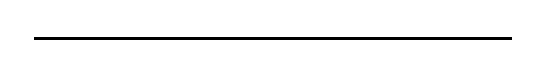
\begin{tikzpicture}
		\draw[thick, black] (0.25*\textwidth, 0) -- (0.75*\textwidth, 0);
		\node[rotate = 360 - 90, xshift = -0.6pt, yshift = 1pt] at (0.25*\textwidth,0){\decotwo};
		\node[rotate = 90, xshift = -0.6pt, yshift = 1pt] at (0.75*\textwidth,0){\decotwo};
	\end{tikzpicture}
	\end{center}
}

\pagestyle{fancy}

\newcommand{\lecday}[1][]
{
    \def\datee{#1}
    \fancyhead[L]{\datee}
}



\newcommand{\signature}
{
	\begin{tikzpicture}[remember picture,overlay]
		\node[fill = YellowOrange!20!white] at ([yshift = 1cm, xshift = -3cm]current page.south east) {\fontsize{10pt}{0pt}{\itshape Kara.$\mathcal{A}$}};
	\end{tikzpicture}
}

\AddToHook{shipout/background}{
  \begin{tikzpicture}[remember picture, overlay]
	  \node[] at ([yshift = 1.5cm,xshift = \textwidth /2 + 0.9cm]current page.south west) {\includegraphics[width = 0.5cm]{preview3}};
	  \node[] at ([yshift = 1.5cm,xshift = - \textwidth /2 - 0.9cm]current page.south east) {\includegraphics[width = 0.5cm]{preview4}};
  \end{tikzpicture}
}



\newtcolorbox[auto counter, number within = section]{remark}[1][]
{
       		title = Remark #1,
		enhanced,
		boxrule = 0pt,
		colback = white,
		breakable,
		arc = 4pt,
		colbacktitle = cyan,
		colback = cyan!5!white,
		segmentation style =
		{
			solid,cyan,thick,
		},
		attach boxed title to top left =
		{
			xshift = 0cm,
		},
		boxed title style =
		{
			boxrule = 0pt,
			sharp corners,
			drop fuzzy shadow = {cyan},
		},
		drop fuzzy shadow = {cyan!80!black},
}

\newtcolorbox[auto counter, number within = section]{theorem}[1][]
{                                      
		title = Theorem \thetcbcounter : #1,
		enhanced, 
		boxrule = 0pt,
		colback = white,
		breakable,
		arc = 4pt,
		colbacktitle = purple,
		colback = purple!5!white,
		segmentation style = 
		{
			solid, purple,thick,
		},
		attach boxed title to top left = 
		{
			xshift = 0cm, 
		},
		boxed title style = 
		{
			boxrule = 0pt,
			sharp corners,
			drop fuzzy shadow = {purple},
		},
		drop fuzzy shadow = {purple!80!black},
}

\newtcolorbox[auto counter, number within = section]{definition}[1][]
{                                      
		title = Definition \thetcbcounter : #1,
		enhanced, 
		boxrule = 0pt,
		colback = white,
		arc = 4pt,
		breakable,
		colbacktitle = YellowOrange!80!black,
		segmentation style = 
		{
			solid, YellowOrange,thick,
		},
		attach boxed title to top left = 
		{
			xshift = 0cm, 
		},
		colback = YellowOrange!5!white,
		boxed title style = 
		{
			boxrule = 0pt,
			sharp corners,
			drop fuzzy shadow = {YellowOrange!80!orange},
		},
		drop fuzzy shadow = {YellowOrange!80!black},
}

\newtcolorbox[auto counter, number within = section]{corollary}[1][]
{                                      
		title = corollary \thetcbcounter : #1,
		enhanced, 
		boxrule = 0pt,
		colback = white,
		arc = 4pt,
		breakable,
		colbacktitle = YellowOrange!80!black,
		segmentation style = 
		{
			solid, YellowOrange,thick,
		},
		attach boxed title to top left = 
		{
			xshift = 0cm, 
		},
		colback = YellowOrange!5!white,
		boxed title style = 
		{
			boxrule = 0pt,
			sharp corners,
			drop fuzzy shadow = {YellowOrange!80!orange},
		},
		drop fuzzy shadow = {YellowOrange!80!black},
}


\newtcolorbox{example}[1][]
{                                      
		title = Example,
		enhanced, 
		boxrule = 0pt,
		colback = white,
		arc = 4pt,
		segmentation style = 
		{
			solid, SpringGreen,thick,
		},
		breakable,
		colback = SpringGreen!5!white,
		colbacktitle = SpringGreen!80!black,
		attach boxed title to top left = 
		{
			xshift = 0cm, 
		},
		boxed title style = 
		{
			boxrule = 0pt,
			sharp corners,
			drop fuzzy shadow = {SpringGreen!80!orange},
		},
		drop fuzzy shadow = {SpringGreen!80!black},
}


\newcommand{\integral}[4]{\int\limits_{#1}^{#2} #4 d#3}
\newcommand{\limit}[3]{\lim\limits_{#1 \rightarrow #2} #3}
\newcommand{\strone}[2]{\left[ \begin{gathered}#1\\ #2\end{gathered} \right] }
\newcommand{\strtwo}[2]{\left\{ \begin{gathered}#1\\ #2\end{gathered} \right\} }
\newcommand{\strthree}[2]{\left\lfloor \begin{gathered}#1\\ #2\end{gathered} \right\rfloor }


\newcommand{\startbf}[1]{\text{\bfseries{#1}}}
\newcommand{\sett}[1]{\left\{ #1 \right\}}
\newcommand{\thesis}[1]{\left( #1 \right)}
\newcommand{\brkt}[1]{\left[ #1 \right]}
\newcommand{\floor}[1]{\left\lfloor #1 \right\rfloor}


\DeclareMathOperator{\img}{im} % Image
\DeclareMathOperator{\Img}{Im} % Image
\DeclareMathOperator{\coker}{coker} % Cokernel
\DeclareMathOperator{\Coker}{Coker} % Cokernel
\DeclareMathOperator{\Ker}{Ker} % Kernel
\DeclareMathOperator{\rank}{rank}
\DeclareMathOperator{\Spec}{Spec} % spectrum
\DeclareMathOperator{\Tr}{Tr} % trace
\DeclareMathOperator{\pr}{pr} % projection
\DeclareMathOperator{\ext}{ext} % extension
\DeclareMathOperator{\pred}{pred} % predecessor
\DeclareMathOperator{\dom}{dom} % domain
\DeclareMathOperator{\ran}{ran} % range
\DeclareMathOperator{\Hom}{Hom} % homomorphism
\DeclareMathOperator{\Mor}{Mor} % morphisms
\DeclareMathOperator{\End}{End} % endomorphism


\newcommand{\lm}{\ensuremath{\lambda}}
\newcommand{\eps}{\ensuremath{\epsilon}}
\newcommand{\veps}{\ensuremath{\varepsilon}}
\newcommand{\al}{\ensuremath{\alpha}}
\newcommand{\bb}{\ensuremath{\beta}}
\newcommand{\cc}{\ensuremath{\gamma}}
\newcommand{\dd}{\ensuremath{\delta}}
\newcommand{\DD}{\ensuremath{\Delta}}
\newcommand{\ff}{\ensuremath{\phi}}
\newcommand{\FF}{\ensuremath{\varphi}}

\newcommand{\RR}{\mathbb{R}}
\newcommand{\RO}{\mathcal{R}}
\newcommand{\EE}{\mathbb{E}}
\newcommand{\CC}{\mathbb{C}}
\newcommand{\RW}{\mathbb{R}^2}
\newcommand{\RT}{\mathbb{R}^3}
\newcommand{\RN}{\mathbb{R}^n}
\newcommand{\DS}{\mathcal{D}}

\newcommand{\KK}{\mathbb{K}}
\newcommand{\KW}{\mathbb{K}^2}
\newcommand{\KT}{\mathbb{K}^3}
\newcommand{\KN}{\mathbb{K}^n}

\newcommand{\NN}{\mathbb{N}}

\newcommand{\PS}{\mathcal{P}}
\newcommand{\AS}{\mathcal{E}}
\newcommand{\FS}{\mathcal{F}}
\newcommand{\LS}{\mathcal{L}}
\newcommand{\MS}{\mathcal{M}}


















\lecday[2025-02-20]

% homeomorphism linear, is isometries in  normed vector spaces i think
% K^n is banach space, why because it's finite dimensional
% therefore $E$ is Banach
% ferme borne sont les compact de l'espace, ist true in metric
% spaces

% \begin{document}
some recap, we have 
\[
\begin{array}{cccc}
        &  \left( \KK^{n}, \| . \| _{\infty } \right)  & \longrightarrow & \left( 
       E,\| . \| _{\infty ,\mathcal{B} }\right) \\
           &
	\begin{pmatrix}
		x_1 \\
		x_2 \\
		 \vdots \\
		 x_{n}\\
	\end{pmatrix}
	   & \longmapsto     &  x_1 e_1 + \hdots + e_{n}x_{n}\\ 
\end{array}
\]
\begin{enumerate}
\item we deduce that $\left( \EE , \| . \| _{\infty , \mathcal{B} } \right)$  is
	banach
\item the compact parts of $\left( E, \| . \| _{\infty} \right)$ 
	are exactly closed and bounded parts  in particular :
\[
S_{E} \left( 0_{E},1 \right) \quad 
\text{ is compact } 
\]
\end{enumerate}
\begin{theorem}[]
On a finite dimensional vector space on $\RR $ or $\CC $, all norms
are equivalent.
\end{theorem}
\begin{proof}
Let $N$ be an arbitrary norm on $E$, we want to show that 
\[
N \sim \| . \| _{\infty ,\mathcal{B} }
\]
we have 
\begin{align*}
	N \left( x \right) = N \left( x_1 e_1 + \hdots + x_{n} e_{n} \right)  
			   & \leq 
			   \sum_{i=1}^{n} 
			   N \left( x_{i} e_{i} \right)  \\
			   &= \sum_{i=1}^{n}  \left| x_{i} \right|
			   N \left( e_{i} \right) 
			   \\
			   & \leq 
			   \left( 
				   \sum_{i=1}^{n} 
				   N \left( e_{i} \right)
			   \right)  \| x \| _{\infty , \mathcal{B} }
\end{align*}                                                    
On the other hand, according to a well known property of the norms
pon a $\KK$-vector space, (See Ex 1.1), 
we have for all $x,y \in E$  :
\[
\left| 
N(x) - N(y) 
\right|
\leq 
N (x-y) 
\]
but since $N \leq \bb  \| . \|_{\infty , \mathcal{B} } $,
we derive that for all $x,y \in E$  : 
\[
\left| N(x) - N(y)  \right| \leq 
\bb  \| x-y \| _{\infty , \mathcal{B} }
\]
implying  that the map :
\[
\begin{array}{cccc}
      N  : &  \left( E, \| . \| _{\infty ,\mathcal{B} } \right)  & \longrightarrow & 
      \left( \RR , \| . \|  \right)\\

           &  x  & \longmapsto     & N(x)  \\ 
\end{array}
\]
is $\bb $-Lipschitz, so continuous on $\left( E, \| . \| _{\infty, \mathcal{B}  } \right)$ 
, next, giving that the unit sphere $S_{E}\left( 0_{E},1 \right)$, of 
$\left( E, \| . \| _{\infty ,\bb } \right)$, is compact in 
$\left( E, \| . \| _{\infty ,\mathcal{B} } \right)$, see properties of the N.V.S
$\left( E,\| . \| _{\infty ,\mathcal{B} } \right)$  cited above, it follows
according to the extreme value theorem, recall 
\divider
\it
Let $X$ be a compact toplogical space and, 
$ f : X \longrightarrow \RR  $ be a continuous map, then 
$f$ is bounded on $X$ and attains its bounds, meaning there exist 
points $x_{min}, x_{\max } \in X$ such that : 
\[
f \left( x_{min} \right) = 
\inf_{x \in X} f(x)  \quad 
\text{ and } \quad 
f(x_{\max })  = \sup_{x \in X}  f(x) 
\]
\divider
\normalfont
that the map $N$ above is bounded on the sphere $S_{E} \left( 
0_{E},1\right)|_{\| . \|_{\infty }, \mathcal{B}}$, and attains 
it's supremum and infinimum in that sphere, so there exist
$x_0 \in S_{E}\left( 0_{E},1 \right)|_{\| . \| _{\infty },\mathcal{B} }$  
such that  
\[
N \left( x \right) \geq N(x_0) \quad 
\left( \forall  x \in S_{E} \left( 0_{E},1 \right)|_{\| . \|_{\infty },\mathcal{B} }
\right)
\]
put $\al := N \left( x_0 \right) \geq 0$ , if we suppose that $\al = 0$, 
we obtain (since $N$ is a norm on $E$) that, 
$x_0 = 0_{E} \notin  S_{E} \left( 0_{E},1 \right)|_{\| . \| _{\infty },
\mathcal{B} }$, which is a contradiction, thus 
$\al > 0$, and we have : 
\[
\forall  x \in S_{E} \left( 0_{E},1 \right)|_{\| . \| _{\infty },\mathcal{B} } 
:
\quad 
N (x)  \geq \al
\]
finally, giving $x \in E \backslash \left\{ 0_{E} \right\}$, by 
applying the last inequality for 
\[
\frac{x}{\| x \| _{\infty ,\mathcal{B} }} 
\in  S_{E} \left( 0_{E},1 \right)
\]
we obtain 
\[
N \left( \frac{x}{\| x \| _{\infty ,\mathcal{B} }} \right) 
\geq  \al
\]
that is 
\[
N \left( x \right) \geq \al \| x \| _{\infty ,\mathcal{B} } 
\quad \left( \forall  x \in E \backslash \left\{ 0_{E} \right\} \right)
\]
this inequality, is also true for $x = 0_{E}$ , hence we get 
\[
N \left( x \right) \geq \al \| x \| _{\infty ,\mathcal{B} } 
\quad  \left( \forall  x \in E \right)
\]
hence we have show that $N$ is equivalent to $\| . \|_{\infty , \mathcal{B} } $,
as required, this completes the proof
\end{proof}
\section{Toplogical and metric properties of a finite-dimensional N.V.S}
From Theorem $1$, we derive several important corollaries. 
\begin{theorem}[]
Let $\KK = \RR $ or $\CC $ , we have : 
\begin{enumerate}[(1)]
	\item Every finite-dimensional N.V.S over $\KK$ is banach
	\item The compact parts of a finite-dimensional 
		N.V.S over $\KK$ are exactly those which are 
		both closed and bounded.
\end{enumerate}
\end{theorem}
\begin{proof}
Let $\left( E,\| . \|  \right)$  be a finite dimensional $N.V.S$, over $\KK$, 
and $n := dim \left( E \right)$, since the case for $n=0$ is trivial, we may
suppose that $n \geq 1$, next let $\mathcal{B} = \left( e_1, e_2, \hdots  \right)$ 
be a basis of $E$, since 
\[
\| . \| \sim \| . \| _{\infty ,\mathcal{B} } \quad 
\text{ by above Theorem } 
\]

then $\left( E, \| . \|  \right)$ has the same
toplogical and metric properties as $\left( E, \| . \| _{\infty ,\mathcal{B} } 
\right)$ so since properties $(1)$ and $(2)$ of the corollary
hold for $\left( E, \| . \| _{\infty ,\mathcal{B} } \right)$  
then they also hold for $\left( E,\| . \|  \right)$, as required this 
achieves the proof.
\end{proof}
\begin{theorem}[]
Let $\KK = \RR $  or $\CC $, and let $E$ and $F$ 
be two $\KK$-N.V.S with $E$ is finite-dimensional, then every
linear mapping from $E$ to $F$ is continuous 
\[
\mathcal{L}  \left( E,F \right) = 
L \left( E,F \right)
\]
\end{theorem}
\begin{proof}
Put $n = dim \left( E \right)$ since the case $n=0$ is trivial, suppose
that $n \geq 1$, fix a basis 
\[
\mathcal{B}  = \left( e_1, \hdots ,e_{n} \right) 
\]
of $E$, let $ f : \left( E,\| . \| _{E} \right) \longrightarrow 
\left( F,\| . \|_{F}  \right)$ be a linear mapping and we will show that
it's continuous, according to Theorem $1$, all norms on $E$ 
are equivalent then in particular 
\[
\| . \| _{E} \sim
\| . \| _{E}
\]
so there exist a positive constant $c$ such that 
\[
\| . \|_{E, \mathcal{B}, \infty  }  
\leq c \| . \| _{E}
\]
using this last inequality together with 
the linearity of $f$ and the properties of a norm on a vector space,
we have for every 
\[
x = x_1 e_1 + \hdots + x_{n}e_{n} \in E \quad 
\left( x_1,x_2, \hdots ,x_{n} \right) \in \KK
\]
we have 
\begin{align*}
\| f(x) \| _{F} =
\| f \left( x_1 e_1 + \hdots + x_{n}e_{n} \right) \| _{F} &=
\| x_1 f\left( e_1 \right) + \hdots + x_{n}f \left( e_{n} \right) \|  
_{F}   \\
							  & \leq 
			\sum_{i=1}^{n} 
			\| x_{i} f(e_{i})  \| _{F} \\
							  &=
							  \sum_{i=1}^{n} 
							  \left| x_{i} \right| 
						\| f(e_{i})  \| _{F} 
							\\
							 & \leq 
						\left( \sum_{i=1}^{n} 
						\| f(e_{i})  \|_{F} \right)
					\| x \| _{E,\infty ,\mathcal{B} } 
					\\
							 & \leq 
							\left( c 
							\sum_{i=1}^{n}
							\| \left( f(e_{i})  \right) \| 
						_{F}
					\right)
					\| x \| _{E}
\end{align*}
that is 
\[
\| f(x)  \| _{F} \leq 
\left( 
	c \sum_{i=1}^{n} 
	\left( f(e_{i})  \right)_{F}
\right)
\| x \| _{E} 
\quad \left( \forall  x \in E \right)
\]
showing that $f$ is continuous, as required
\end{proof}
\divider
we have also the following important theorem 
\begin{theorem}[]
Let $E$ and $F$ be two N.V.S over $\KK \left( 
	\left\{ \RR ,\CC  \right\}
\right)$, with $F$ is Banach, then the $\KK$-N.V.S 
$\mathcal{L} (E,F) $  is Banach.
\end{theorem}
\begin{proof}
	We have to show that any Cauchy sequence 
	of $\mathcal{L} \left( E,F \right)$  
	is convergent in $\left( \mathcal{L} (E,F)  \right)$  
	so let $\left( f_{n} \right)_{n \in \NN}$  be a Cauchy sequence
	of $\mathcal{L} (E,F) $ and let us show that it converges for some
	$f \in \mathcal{L} (E,F) $, by hypothesis, we have :
	\[
	\forall  \veps  >  0, \exists  N = N(\veps) \in 
	\NN,
	\forall p,q \in \NN : \quad  
	p > q \geq N \implies 
	\mid \mid \mid  f_{p} - f_{q} \mid \mid \mid  \leq \veps 
	\]
	it follows from the definition of the norm 
	$\mid \mid \mid  . \mid \mid \mid $  of 
	$\mathcal{L}(E,F)  $ that : 
	\[
	\forall \veps  > 0, \exists 
	N = N(\veps )  \in \NN, \forall p,q \in \NN : 
	\quad p > q \geq N \implies 
	\forall x \in E : 
	\quad \| f_{p}(x) - f_{q}(x)   \|  \leq \veps  
	\| x \| _{E}
	\]
	for $x \in E \backslash \left\{ 0_{E} \right\}$  fixed, 
	by taking instead of $\veps $  the positive
	real number 
	$\frac{\veps }{\| x \|_{E} }$, we desire the following 
	\[
	\forall \veps  > 0, \quad N \left( \veps ,x \right) 
	\in \NN, \forall p,q \in \NN : 
	\quad p > q \geq N \left( \veps , x \right) 
	\implies 
	\| f_{p}(x) - f_{q}(x)   \|  _{F} \leq 
	\veps 
	\]
	show that, for all $x \in E \backslash \left\{ 0_{E} \right\}$ 
	the sequence  $\left( f_{n} (x) \right)_{n \in \NN}$  of 
	$F$ is Cauchy, since $F$ is Banach then for all 
	$x \in E \backslash \left\{ 0_{E} \right\}$, the sequence 
	$\left( f_{n} \right)_{n \in \NN}$ of $F$ is convergent, 
	remark that the same sequence $\left( f_{n}(x)\right)_{n \in \NN}$ 
	of $F$ also converge for $x = 0_{E}$ to $0_{F}$, since
	$f_{n}(0_{E})=0_{F} $ , then for all $n \in \NN$ , because the 
	maps $f_{n}$ are all linear so let us define 
	\[
	\begin{array}{cccc}
	      f : &  E  & \longrightarrow & F \\
	
	           &  x  & \longmapsto     & f(x) := 
		   \lim_{n \to \infty } f_{n}(x) \\ 
	\end{array}
	\]
	Now, we are going to show that $f \in \mathcal{L}(E,F)$, 
	that is $f$ is linear and continuous, and that $f$ 
	is the limit of the sequence $\left( f_{n} \right)_{n \in \NN}$  in 
	$\mathcal{L} (E,F)$
	\begin{center}
		\it is $f$  linear? 
	\end{center}
	\normalfont
	for all $x, y \in E$, for all $\lm \in \KK$, we have 
	\begin{align*}
		f \left( \lm x + y \right) & := 
		\lim_{n \to \infty } 
		f_{n}(\lm x + y)  \\
					   & =
					   \lim_{n \to \infty } 
					  \left( 
						  \lm f_{n}(x) + 
						  f_{n}(y) 
					  \right) \hfill
					  \text{ since $f_{n}$ is 
					  linear for all $n \NN$ } \\
					   &= 
					   \lm\lim_{n \to \infty} f_{n}(x)  
					   + 
					   \lim_{n \to \infty }  f_{n}(y)  
					   \hfill 
					   \left( \text{ by the continiouty 
					   of law $+$ and $.$ of $F$   }  \right)
					   \\
					    & =
					    \lm f(x)  + f(y)  
	\end{align*}
	implying that $f$ is linear
	\begin{center}
		\it is $f$ continuous?
	\end{center}
	\normalfont
		\normalfont By taking in 
		$\veps  = 1$ , $q = N = N (1) \in \NN $, and by letting
		$p \rightarrow \infty $, we obtain according to the continiouty
		of the norm $\| . \| _{F}$, that 
		\begin{align*}
			\| f(x) - f_{N}(x)  \|  & \leq 
			\veps  \| x \| _{E} \quad 
			\left( \forall  x \in E \right) \\
			\| \left( f- f_{N}  \right)(x)  \|  & \leq 
			\| x \| _{E} \quad 
			\left( \forall  x \in E \right)
		\end{align*}
		which implies that the linear map $\left( f-f_{N} \right)$, from 
		$E$ to $F$ is continuous, thus $f := f_{N} + \left( f-f_{N} \right)$ 
		is also continuous as the sum of two continuous 
		mappings, consequently : 
		\[
		f \in \mathcal{L} (E,F)  
		\]
		\begin{center}
			\it
			is $f$ the limit of $\left( f_{n} \right)_{n \in \NN}$  
			in $\mathcal{L}(E,F) $ 
		\end{center}
		\normalfont
		\[
		\forall  \veps  > 0, \exists N= N(\veps )  
		\in \NN, 
		\forall p,q \in \NN: \quad 
		p > q \geq N \implies 
		\forall  x \in E : 
		\| f_{p}(x) - f_{q}(x)   \|  _{F} \leq 
		\veps  \veps  \| x \|_{E}
		\]
		by letting $p \rightarrow \infty $, and taking into account
		the continiouty of the norm $\| . \| _{F}$  of $E$, we obtain that
		\begin{align*}
		\forall \veps  > 0, \exists N = N(\veps )  \in \NN, 
		\forall q \in \NN: \quad  
		q \geq N &\implies 
		\forall x \in E : 
		\| f_{p}(x) - f(x)   \|  \leq 
		\veps  \| x \| _{E} \\
		& \iff \forall  x \in E : 
		\quad \frac{\| \left( f_{q}-f \right)(x)  \| _{F}}{ \| x \| _{E}} 
		\leq  \veps 
		\end{align*}
		that is 
		\[
		\forall  \veps  > 0, \exists  N = N \left( \veps  \right) \in \NN, 
		\forall  q \in  \NN : \quad 
		q \geq N \implies 
		\sup_{x \in E \backslash \left\{ 0_{E} \right\}}  
		\frac{\| \left( f_{q}-f \right)(x)  \|_{F} }{
			\| x \|_{E}
		} \leq \veps 
		\]
		that is 
		\[
		\forall  \veps  > 0, \exists N = N(\veps )  \in \NN, 
		\forall q \in \NN : 
		\quad q \geq N \implies 
		\mid \mid \mid  f_{q} - f \mid \mid \mid  \leq \veps 
		\]
		showing that the sequence 
		$\left( f_{n} \right)_{n \in \NN}$  
		converges to $f$ in $\mathcal{L} \left( E,F \right)$, this completes
		the proof
\end{proof}
% \end{document}
